\documentclass[12pt]{ctexart}
\usepackage{amsmath,graphicx,textcomp,subfigure,indentfirst,ctex,color,float}
\title{Lecture 4}
\author{赵思逸}

\date{\today}
\newcommand{\new}[1]{\textcolor{blue}{#1}}

\newcommand{\refeq}[1]{式~(\ref{#1})}

\begin{document}

\maketitle

\new{\section*{CMB坐标系}}


\new{
我们上节课得到的FRW度规基于“宇宙学坐标系”,在实际操作层面,我们用相对于CMB静止的坐标系作为“宇宙学坐标系”。  
太阳绕CMB运动的dipole速度经测量为370km/s,在CMB上体现为 $\frac{v}{c} \sim 10^{-3}$ 的涨落。
虽然我们的太阳系并不是“宇宙学坐标系”,但仍不影响我们使用FRW度规研究宇宙学,类似于在平地上研究火车上的物理学,只差一个坐标变换。
}

\section{宇宙学中的距离}

\subsection{角直径距离(angular diameter distance) $d_A$ }

给定“标准尺子”(物理长度固定为$l$且已知)。
在静止宇宙中,距离 $r = l/\theta$ ,其中 $\theta$ 是“标准尺子”的张角。
一般情况下,定义角直径距离
\begin{equation}
    d_A \equiv l/\theta
\end{equation}

在膨胀的平直宇宙(K=0)中,假设“标准尺子”在t时刻发出的光今天被我们看到。
因为宇宙均匀膨胀,$\theta$角固定不变。
在t时刻,“标准尺子”距离我们$a(t)r$,其中$r$是共动坐标系下的坐标距离。
在今天,“标准尺子”距离我们$a_0 r$。
由此得知
\begin{equation}
    \theta = \frac{l}{a(t)r} = \frac{l a_0/a(t)}{a_0 r}
\end{equation}
\begin{equation}
    d_A \equiv \frac{l}{\theta} = \frac{a(t)}{a_0} a_0 r = a(t) r
\end{equation}

\subsection{光度距离(luminosity distance) $d_L$ }

假设某标准烛光(standard candle)发出单频光,
已知其亮度 $L=\frac{\Delta E}{\Delta t} = \frac{h\nu \Delta N}{\Delta t}$,
观测到流量 $F=\frac{\Delta L}{\Delta A} = \frac{L}{4\pi r^2}$.
在静止宇宙中,该标准烛光的距离为 $r=\sqrt{\frac{L}{4\pi F}}$.
一般情况下,定义光度距离
\begin{equation}
    d_L \equiv \sqrt{\frac{L}{4\pi F}}
\end{equation}

在膨胀的平直宇宙(K=0)中,假设标准烛光在t时刻发出的光今天被我们看到。
其亮度$L=\frac{\Delta E_\text{em}}{\Delta t_\text{em}} = \frac{h\nu_\text{em} \Delta N_\text{em}}{\Delta t_\text{em}}$。

$\Delta N$不变的情况下,由于宇宙膨胀,接受这些光子所需的时间变长 $\Delta t = \Delta t_\text{em}\frac{a_0}{a(t)}$。
同时光子的波长被拉长,频率下降$\nu=\nu_\text{em}\frac{a(t)}{a_0}$,
导致$\Delta E = h\nu\Delta N=\frac{a(t)}{a_0}h \nu_\text{em} \Delta N_\text{em}$。

观测到的亮度 $L_\text{obs}=\frac{\Delta E}{\Delta t}=\left(\frac{a(t)}{a_0}\right)^2 L$,
观测到的流量
\begin{equation}
    F=\frac{L_\text{obs}}{4\pi (ra_0)^2}=\left(\frac{a(t)}{a_0}\right)^2 \frac{L}{4\pi r^2 a_0^2}
\end{equation}

得到光度距离
\begin{equation}
    d_L\equiv\sqrt{\frac{L}{4\pi F}}= \left(\frac{a_0}{a(t)}\right)a_0 r 
\end{equation} 

\subsection{弯曲宇宙中的距离}

以$K=1$为例,我们有两种共动距离:
\begin{itemize}
    \item $r$ 是共动坐标系下的三维投影空间的坐标距离
    \item $\chi_\text{com}$ 是光传播经过的共动距离
\end{itemize}

对于一段弧(比如标准尺子), $dt=dr=d\phi = 0$ , $ds^2=a^2(t)r^2d\theta^2$ ,
\begin{equation}
    d_A\equiv \frac{l}{d\theta} = \frac{ds}{d\theta} = a(t)r
\end{equation}

\begin{figure}[!hbtp]
    \centering
    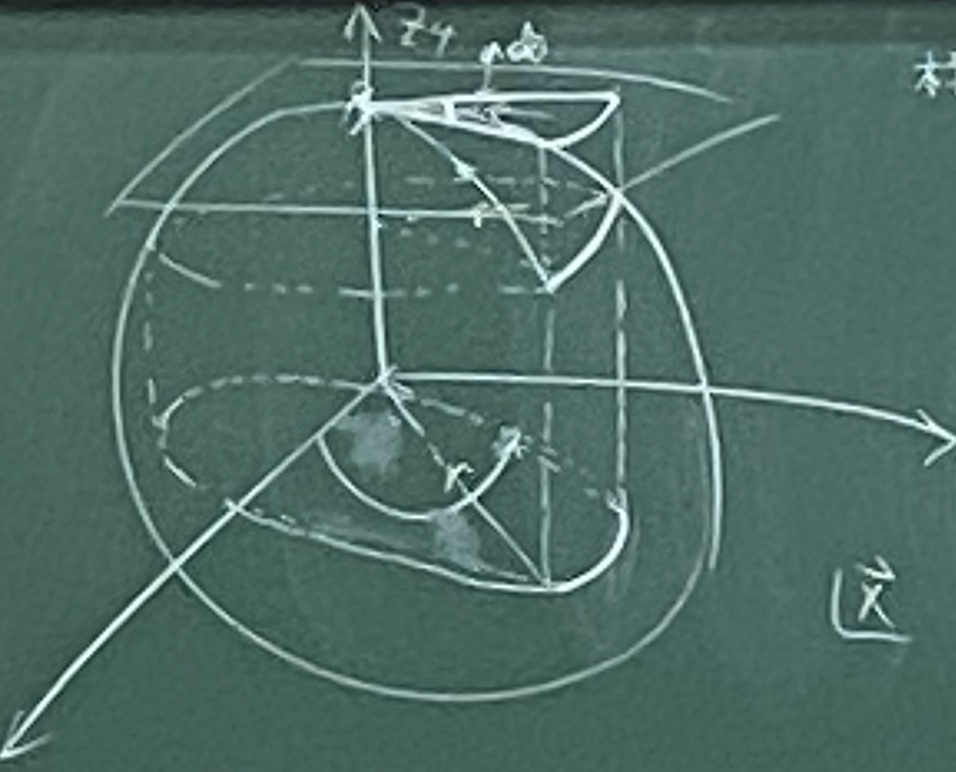
\includegraphics[width=0.8\textwidth]{figures/d_A.png}
    \caption{弯曲空间中的角直径距离示意图,观测者在极点。}
\end{figure}

对于一个立体角, $dt=dr=0$ , $ds^2=a^2(t)r^2d\Omega^2$ ,球面积 $=a^2(t) 4\pi r^2$ 
\begin{equation}
    F = \frac{L_\text{obs}}{a_0^2 4\pi r^2}
\end{equation}
\begin{equation}
    d_L\equiv \frac{a_0}{a}a_0 r
\end{equation}

\begin{figure}[!hbtp]
    \centering
    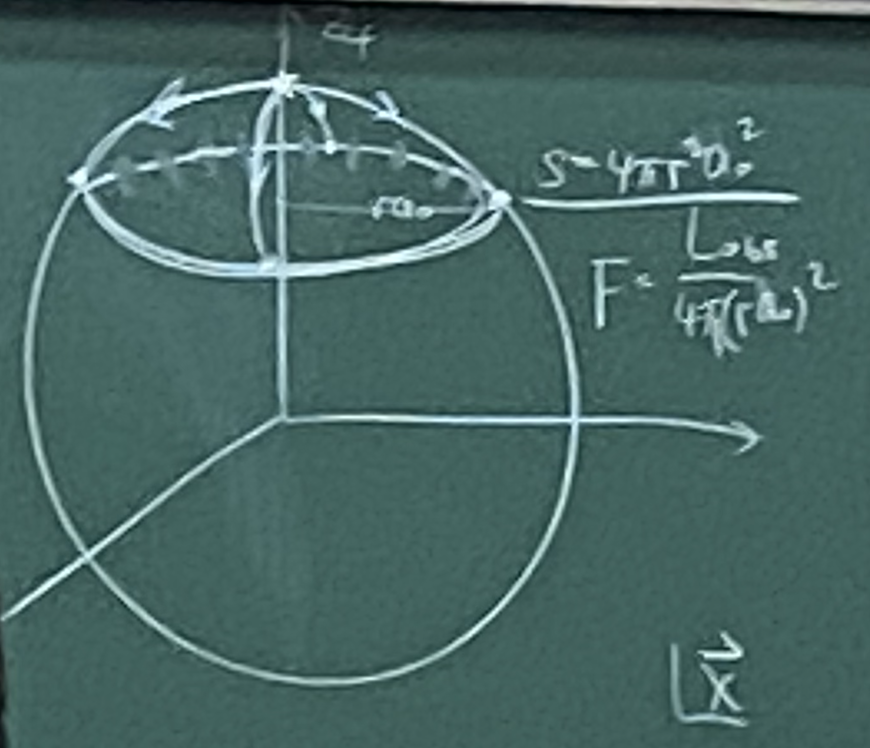
\includegraphics[width=0.8\textwidth]{figures/d_L.png}
    \caption{弯曲空间中的光度距离示意图吗,光源在极点。}
\end{figure}


\subsection*{consistency check}
由 $d_A$ 和 $d_L$ 可以得到与宇宙学模型无关的“consistency check”:
\begin{equation}
    \frac{d_A}{d_L} = \left(\frac{a}{a_0}\right)^2 = \frac{1}{(1+z)^2}
\end{equation}  
这个公式可以用来检验“宇宙均匀膨胀”的假说。

定义 $\chi$ 是光传播经过的空间对应在今天的(物理)距离
\begin{eqnarray}
    \chi &=& \chi_\text{com} a_0 \\
        &=& \int_t^{t_0} c dt^\prime \frac{a_0}{a(t^\prime)} \label{eq:chidefine} \\ 
        &=& a_0 \int_0^r \frac{dr^\prime}{\sqrt{1-Kr^{\prime 2}}}
\end{eqnarray}
最后一个等号是因为对于光线来说,$ds^2=0$, $d\theta=d\phi = 0$ ,因此 $\frac{c dt}{a(t)}=\frac{dr}{\sqrt{1-Kr^2}}$ 。结果是
\begin{equation}
    \chi = a_0 \times
    \begin{cases}
        \sin^{-1} r & K=+1 \\ 
        r & K=0 \\ 
        \sinh^{-1} r & K=-1
    \end{cases}
\end{equation}

由此得知共动坐标距离
\begin{equation}
    r = S_k(\chi/a_0)
\end{equation}
其中
\begin{equation}
    S_k(x) = 
    \begin{cases}
        \sin{x} & K=+1 \\ 
        x & K=0 \\ 
        \sinh{x}  & K=-1
    \end{cases}
\end{equation}

而$\chi$可以根据定义(\refeq{eq:chidefine})计算
\begin{eqnarray}
    \chi &=& \int_t^{t_0} c dt^\prime \frac{a_0}{a(t^\prime)} \\
        &=& \int_{a/a_0}^{1}  \frac{c da^\prime}{a^{\prime 2}H(a^\prime)} \\
        &=& \int_{0}^{z}  \frac{c dz^\prime}{H(z^\prime)} \label{eq:z2chi}
\end{eqnarray}

使用\refeq{eq:z2chi}可以计算任意红移下的距离,注意其中$H(z^\prime)$具体的形式与宇宙学模型有关,接下来的课我们会讲$H(z^\prime)$的具体形式是什么。


\end{document}
